\section{Lecture 30 - 11/16/2022}

\subsection{Harmonic Conjugates}

\begin{definition}
    Let $\Omega$ be a domain and real-valued $u \in \text{Harm}(\Omega)$, suppose there exist real-valued $v \in \text{Harm}(\Omega)$ such that
    \[u + iv \in \text{Hol}(\Omega)\]
    then $v$ is called the \textbf{harmonic conjugate} of $u$ and we denote $\Tilde{u} \coloneqq v$. In particular, note that $\Tilde{v} = -u$. Note that all complex conjugates of $u$ \underline{differ by a constant}.
\end{definition}

\begin{theorem}
    If $\Omega$ is a simply connected domain, then harmonic conjugates always exist.
\end{theorem}

\begin{proof}
    Let $u \in \text{Harm}(\Omega)$, then by the Cauchy-Riemann Equation, it suffices to find $v \in \text{Harm}(\Omega)$ satisfying:
    \[\frac{\partial u}{\partial x} = \frac{\partial v}{\partial y}, \frac{\partial u}{\partial y} = -\frac{\partial u}{\partial x}\]
    Or equivalently that
    \[dv = \frac{\partial v}{\partial x} dx + \frac{\partial v}{\partial y} dy = - \frac{\partial u}{\partial y} dx + \frac{\partial u}{\partial x} dy\]
    Now fix $z_0 \in \Omega$, then we claim that
    \[v(\xi) = a + \int_{z_0}^\xi - \frac{\partial u}{\partial y} dx + \frac{\partial u}{\partial x} dy\]
    is our desired function. Note that $v$ is well-defined since $\Omega$ is simply connected. Now clearly $u + iv$ is holomorphic, so it remains for us to show that $v$ is harmonic:
    \begin{align*}
        d(dv) &= d(- \frac{\partial u}{\partial y} dx + \frac{\partial u}{\partial x} dy)\\
        &= -\frac{\partial^2 u}{\partial y^2} dy \wedge dx + \frac{\partial^2 u}{\partial x^2} dx \wedge dy\\
        &= (\Delta u) dx \wedge dy\\
        &= 0 \tag*{$u$ is harmonic}
    \end{align*}
\end{proof}

\begin{remark}
    The assumption that $\Omega$ is simply connected is essential. Consider the following example:
    \[u(z) = \ln |z| \text{ on } r < |z| < R\]
    We claim that $u$ does not have any harmonic conjugates.
\end{remark}

\begin{proof}
Suppose a conjugate $v$ does exist, then
\[dv = - \frac{\partial u}{\partial y} dx + \frac{\partial u}{\partial x} dy\]
Let $r'$ be between $r$ and $R$ and $C_{r'}$ be the circle centered at origin of radius $r'$, since $C_{r'}$ is a closed loop, endpoints match, so
\[\int_{C_{r'}} - \frac{\partial u}{\partial y} dx + \frac{\partial u}{\partial x} dy = 0\]
However, evaluating the integral explicitly gives us that 
\[- \frac{\partial u}{\partial y} dx + \frac{\partial u}{\partial x} dy \neq 0\]
\end{proof}

\begin{question}
    Let $\Dbb$ be the unit disk. Suppose $u \in \text{Harm}(\Dbb) \cap C(\overline{\Dbb}^{cl})$, then we know $u$ contains a harmonic conjugate $v$. How can we describe $u + iv$ explicitly?
\end{question}

\begin{proof}[Idea]
The idea is to find $S(z) \in \text{Hol}(\Dbb)$ such that
\[P(z) = \text{Re}(S(z))\]
, where $P(z)$ is the Poisson Formula. Then we have that
\[f(z) = \int_{\Tbb} S(z \overline{\xi}) u(\xi) \frac{|d\xi|}{2\pi}\]
Note that $f$ is analytic by Morera's Theorem and
\[\text{Re}(f(z)) = \int_{\Tbb} P(z \overline{\xi}) u(\xi) \frac{|d\xi|}{2\pi} = u(\xi)\]
So, how do we find this desired $S(z)$? Recall that
\[P(z) = 1 + \sum_{k \geq 1} z^k + \sum_{k \geq 1} \overline{z}^k\]
Then choosing
\begin{align*}
    S(z) &\coloneqq 1 + 2 \sum_{k \geq 1} z^k\\
    &= 1 + \frac{2z}{1 - z} \tag*{Domain of $S(z)$ is $\Dbb$}\\
    &= \frac{1 + z}{1 - z}
\end{align*}
will suffice. $S(z)$ is sometimes called the \textbf{Schwartz Kernel}.\\\\
Now let $Q(z) = \text{Im}(S(z))$, then
\[v(z) = \text{Im}(f(z)) = \int_{\Tbb} Q(z \xi) u(\xi) \frac{|d\xi|}{2\pi}\]
So we have that
\begin{align*}
    f(z) &= u(z) + i v(z)\\
    &= \int_{\Tbb} u(\xi) \frac{1 + z \overline{\xi}}{1 - z \overline{\xi}} \frac{|d\xi|}{2\pi}\\
    &= \int_{\Tbb} u(\xi) \frac{\xi + z}{\xi - z} \frac{|d\xi|}{2\pi}
\end{align*}
\end{proof}

\subsection{Reflection Principle for Analytic Functions}

Let $\Omega = \Omega^*$ be a symmetric domain and $f \in \text{Hol}(\Omega^+)$ such that
\[\lim_{z \to \xi} \text{Im}(f(z)) = 0,\ \forall \xi \in \Rbb \cap \Omega\]
(recall previously we assumed that the limit to the real part exists) 

Let $f = u + iv$. Recall the reflection principle allowed us to extend $v$ harmonically to
\[\Tilde{v}(z) = \begin{cases}
    v(z),\ z \in \Omega^+\\
    0,\ z \in \Rbb \cap \Omega\\
    -u(\overline{z}),\ z \in \Omega^-
\end{cases}\]

We can extend u to $\Tilde{u}$ on $\Omega \setminus \Rbb$ as
\[\Tilde{u}(z) = \begin{cases}
    u(z),\ z \in \Omega^+\\
    u(\overline{z}),\ z \in \Omega^-
\end{cases}\]

Altogether, this extends $f$ to a function $\Tilde{f} \in \text{Hol}(\Omega \setminus \Rbb)$.\\

For a particular $\xi_0 \in \Rbb$, consider the diagram:
\[\fbox{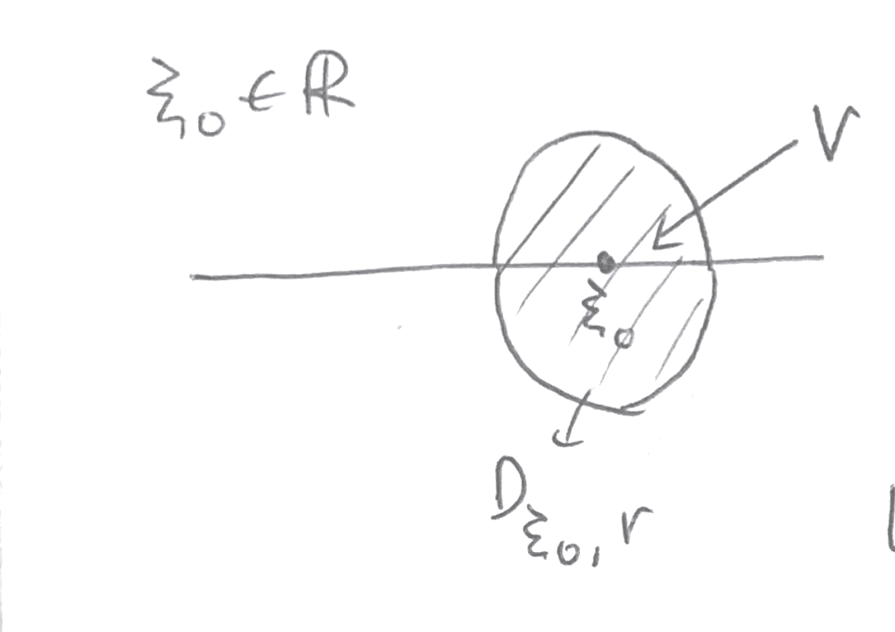
\includegraphics[width=.8\textwidth]{Figures/reflection_pricp.png}}\]

Let $u, v$ be harmonic on the upper-half disk as before, and let $\Tilde{v}$ be the extension of $v$ and $v'$ be the harmonic conjugate, then
\[-v' + i\Tilde{v} \in \text{Hol}(D_{\xi_0, r})\]

We can choose $v'$ to be symmetric ($v'(z) = v'(\overline{z})$ (Follows from the Schwartz Kernel Formula), then it follows that
\[-v'(z) = u(z) + C, \forall z \in D_{\xi_0, r}^+\]

\subsection{Liouville's Theorem for Harmonic Functions}

\begin{theorem}[Liouville's Theorem for Harmonic Functions]
    Let $u \in \text{Harm}(\Cbb)$, if for all $z \in \Cbb$, $|u(z)| \leq C < \infty$, then $u(z)$ is identically constant.
\end{theorem}

The proof of this theorem relies on the following lemma:

\begin{theorem}[Harnack's Inequality]
    If $u \in \text{Harm}(D_{0, R})$ and $u \geq 0$ is non-negative, then for any $|z| \leq r < R$,
    \[\frac{R - r}{R + r} u(0) \leq u(z) \leq \frac{R + r}{R - r} u(0)\]
\end{theorem}

\begin{proof}[Proof of Harnack's Inequality]
    If $R = 1$, then consider $u \in \text{Harm}(\Dbb) \cap C(\overline{D}^{cl})$, then we can write
    \[u(z) = \int_{\Tbb} \frac{1 - |z \overline{\xi}|^2}{|1 - z \xi|^2} u(\xi) \frac{|d\xi|}{2\pi}\]
    , where we know that $\xi$ takes values from $\Tbb$ the unit circle, so
    \begin{align*}
        \frac{1 - |z \overline{\xi}|^2}{|1 - z \xi|^2} &\leq \frac{(1 - |z|)(1 + |z|)}{(1 - |z|)^2}\\
        &= \frac{1 + |z|}{1 - |z|}\\
        &\leq \frac{1 + r}{1 - r} \tag*{Since $|z|$ is monotonic}
        \frac{1 - |z \overline{\xi}|^2}{|1 - z \xi|^2} &\geq \frac{(1 - |z|)(1 + |z|)}{(1 + |z|)^2}\\
        &= \frac{1 - |z|}{1 + |z|}\\
        &\geq \frac{1 - r}{1 + r} \tag*{Since $|z|$ is monotonic}
    \end{align*}
    So we have the inequality
    \[\frac{R - 1}{R + 1} u(0) \leq u(z) \leq \frac{R + 1}{R - 1} u(0)\]
    Now for a general $R$, consider
    \[u_a(z) = u(az), a < R\]
    Then we will eventually get the inequality that
    \[\frac{a - r}{a + r} u(0) \leq u(z) \leq \frac{a + r}{a - r} u(0)\]
    Then we can take the limit as $a \to R$.
\end{proof}

Now we are ready to prove Liouville's Theorem for Harmonic Functions:

\begin{proof}
    Let $|z| \leq r$, we can without loss replace $u$ by $u + C$ so that $u$ is non-negative (we can do this because $u$ is bounded). So Harnack's Inequality gives us that
    \[\frac{R - r}{R + r} u(0) \leq u(z) \leq \frac{R + r}{R - r} u(0)\]
    Taking $r \to \infty$ on both sides gives us that
    \[u(0) \leq u(z) \leq u(0),\ \forall z \in \Cbb\]
\end{proof}